\documentclass[smallheadings,12pt]{scrartcl}

\usepackage{listings}
%\usepackage[pdftex]{graphicx}

\title{Python Exercises\\Introduction - Simple}
\date{}
\lstset{language=Python,numbers=left,frame=shadowbox}

\begin{document}
\maketitle
\section{Simple arithmetic}
\begin{itemize}
\item 3/5 + 2
\item 3/float(5) + 2
\item 3/5. + 2
\item 3/5 + 2.
\item 3**2
\item 3**(2+5)
\item (3**2)+5
\item 3./5/2
\item 3/5/2.
\item 3/5./2
\item 5\%2
\end{itemize}
\pagebreak

\section{Script}
Create a .py file with the following content and make sure you understand every line. Execute it.

\begin{lstlisting}
#!/usr/bin/env python
#
# A program for numbers
#

a = 3 - 4 + 10
b = 5 * 6
c = 7.0/8.0
print "Hello World, these are the values:", a, b, c
print "Increment", a, "by one: "
a = a +1
print a
print "The sum of", a, "and", b, "is?"
a = ' are'
b = "you"
c = "years old. Don't you think?"
d = b + a
number = raw_input("Input a number ")
print d, number, c
\end{lstlisting}

N.B.: sometimes one finds input instead of raw\_input. Please be very careful using input because input is equivalent to eval(raw\_input(prompt)), thus implies:
\begin{itemize}
\item Exceptions are raised for non-well-formed Python expressions, and, more ominously,
\item Well formed Python expressions can wreak havoc. The user could, after all, type a string consisting of the Python expressions to delete all files from an arbitrary directory on the system.
\end{itemize}


\section{Logical expressions}

\begin{enumerate}
\item For the following expressions, replace a, b, c with 1 or 0 so that the expression becomes true (i.e. 1). Use the Python interpreter. Which expressions are logically equivalent? %Record some of your results in truth tables.
\begin{enumerate}
\item (a and b)
\item (not a and b)
\item (not (a and b))
\item (a or b)
\item (a or not b)
\item (not (a or b))
\item (not (not a or not b))
\item (a and (a or b))   Does this really depend on b?
\item (a and b and c)
\item (a and b or c)
\item (a and (b or c))
\item ((a and b) or c)
\end{enumerate}
\item Write a script that asks someone to input their first name, last name and phone number. If the user does not type at least some characters for each of these, print "Do not leave any fields empty" otherwise print "Thank you". (Hint: if a variable is empty, its value will be "false".)
\item Write a program that asks a user to input a number. If the number equals "5", output "My lucky number". If the number is larger than 10, output "What a large number!". In all other cases, output "That's not my lucky number."
\item Objects can have equal values or can be identical. A test for having equal values is ==; a test for being the same object is \textit{is}. For example define a = 5, b = 5.0 and c = a. Try the following:
\begin{itemize}
\item \textit{a == b}
\item \textit{a is b}
\item \textit{a is c}
\end{itemize}

\end{enumerate}


\section{Program flow}
\begin{enumerate}
\item Make a 'for' loop that sums '1' hundred times.
\item Make a 'for' loop that sums the numbers from 1 to 100. Change the code to sum only the odd numbers.
\item Make a variable word1='gateman'. Make a for loop that inverts the letter order of word1.
%\item Write the codes that produce the depicted program flows:\\
%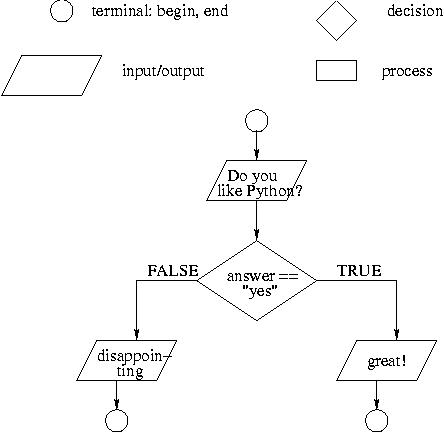
\includegraphics[scale=0.5]{./pics/p21.jpg}
%
%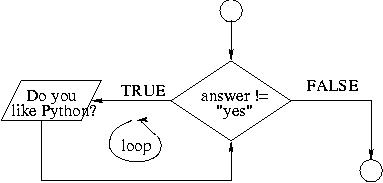
\includegraphics[scale=0.5]{./pics/p22.jpg}
\end{enumerate}


\section{Lists}

\begin{enumerate}
\item "Flatten" a list of lists.
for example: [ [a,b,c],[d,e],[f] ] $\rightarrow$ [ a,b,c,d,e,f ]
\item Create a list that contains the names of 5 famous persons. Print the list. Ask the user to input one more name and append it to the list. Print the list. Ask a user to input a number. Print the name that has that number as index. Add "Mario" and "Luigi" at the beginning of the list (by using "+"). Print the list. Remove the last name from the list. Print the list. Ask a user to type a name. Check whether that name is in the list: if it is then delete it from the list. Otherwise add it at the end. Create a copy of the list in reverse order. Print the original list and the reverse list. Well done!
\item Use the list of celebrity names from the previous exercise: Create a for loop that prints for each name "hello ceb\_name, how are you?" where ceb\_name is replaced by the name of the celebrity.
\item Please open the file list1.py and follow the instructions.
After you are done, there is also list2.py.
\end{enumerate}
\end{document}
